
\documentclass[a4paper,12pt]{article}
\usepackage[utf8]{inputenc}
\usepackage{geometry}
\geometry{a4paper, margin=1in}
\usepackage{graphicx}
\usepackage{booktabs}

\title{Task 4: Insights and Recommendations for Fintech Reviews}
\author{}
\date{June 11, 2025}

\begin{document}

\maketitle

\section{Insights}
\subsection{Drivers and Pain Points}
\begin{itemize}
  \item \textbf{Commercial Bank of Ethiopia}: Driver - "App Usability" (135 reviews, e.g., "proactive", "good"); Pain Point - "Transaction Problems" (20 reviews, e.g., "not functional", "send").
  \item \textbf{Bank of Abyssinia}: Driver - "App Usability" (146 reviews, e.g., "app", "UI"); Pain Point - "Login Issues" (17 reviews, e.g., "error", "sign").
  \item \textbf{Dashen Bank}: Driver - "App Usability" (207 reviews, e.g., "intuitive", "superapp"); Pain Point - "Transaction Problems" (60 reviews, e.g., "slow").
  \item \textbf{Comparison}: Abyssinia has the highest negative sentiment (226), Dashen the highest positive (297).
\end{itemize}

\subsection{Recommendations}
\begin{itemize}
  \item Add a budgeting tool to enhance "App Usability" across all banks.
  \item Implement transaction recovery for CBE and Dashen.
  \item Address "Login Issues" with crash recovery for Abyssinia.
  \item Optimize performance for Dashen to reduce "Transaction Problems."
\end{itemize}

\section{Visualizations}
\begin{figure}[h]
  \centering
  \includegraphics[width=0.8\textwidth]{visuals/sentiment_trends_monthly.png}
  \caption{Sentiment Trends Over Time (Monthly)}
\end{figure}
\begin{figure}[h]
  \centering
  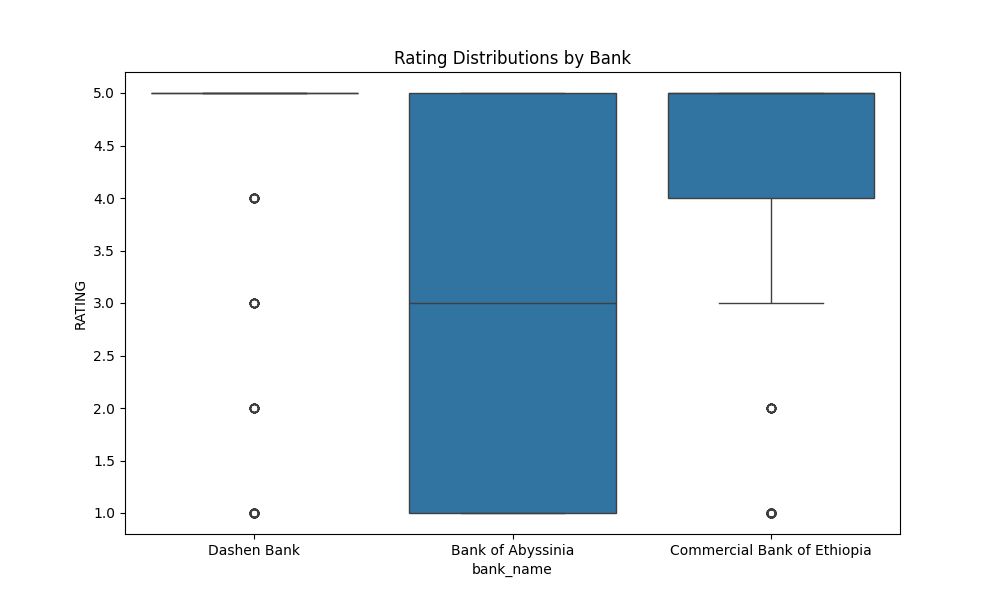
\includegraphics[width=0.8\textwidth]{visuals/rating_distributions.png}
  \caption{Rating Distributions by Bank}
\end{figure}
\begin{figure}[h]
  \centering
  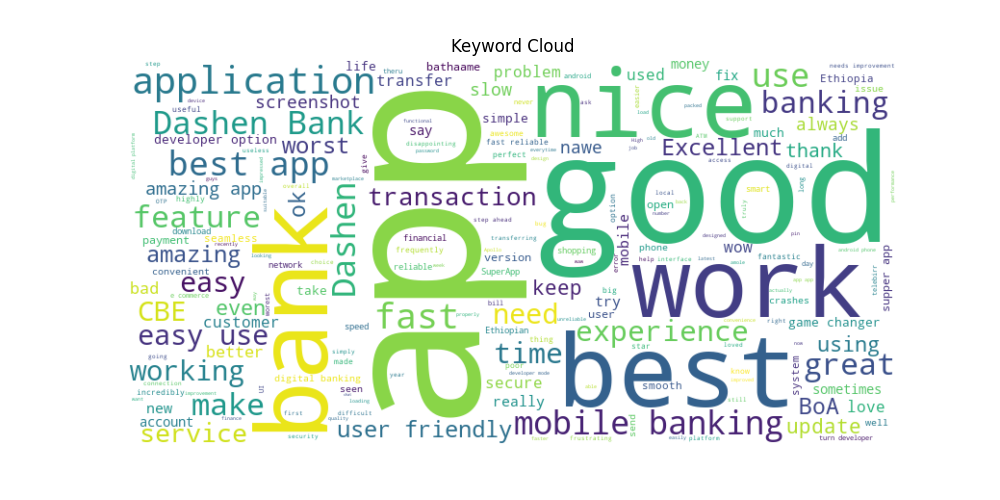
\includegraphics[width=0.8\textwidth]{visuals/keyword_cloud.png}
  \caption{Keyword Cloud}
\end{figure}

\section{Ethical Considerations}
Negative feedback may dominate due to dissatisfied users, potentially skewing theme analysis.

\section{Conclusion}
The analysis identifies key drivers and pain points, supported by visualizations, with ethical biases noted.

\end{document}
